% vim:set textwidth=100:
% vim:set fo+=t:

\documentclass[12pt]{article}

\usepackage{amsmath}
\usepackage[nofiglist,notablist]{endfloat}
\usepackage[usenames,dvipsnames]{color}
\usepackage{color}
\usepackage{authblk}
\usepackage{graphicx}
\usepackage{palatino}
\usepackage[activate={true,nocompatibility},final]{microtype}
\usepackage[super,sort&compress]{natbib}
\pagenumbering{arabic}
\parskip = 0.08in \parindent = 0.0in

% Custom macros for author comments
\newcommand{\Alberto}[1]{\color{ForestGreen}#1\normalcolor }
\newcommand{\Justin}[1]{\color{blue}#1\normalcolor}
\newcommand{\Arijit}[1]{\color{magenta}#1\normalcolor}
\newcommand{\Ken}[1]{\color{red}#1\normalcolor}

\author{Arijit~Roy}
\author{Alberto~Perez}
\author{Ken~A.~Dill}
\author{Justin~L.~MacCallum}
\affil{Laufer Center for Physical and Quantitative Biology\\
    and Departments of Physics and Chemistry\\
    Stony Brook University\\
    Stony Brook, NY 11794-5252.}

\title{Predicting the conformational preferences of proteins using a physics-based free energy
method}

\begin{document}

\maketitle

\begin{abstract}


Understanding the free energy differences between different conformations of a protein is important for
understanding biochemical mechanisms. The calculation of such free energy differences is difficult and
computationally demanding. In this work, we explore the use of the "confinement method'' to calculate free energy
differences between conformations. This method provides two main advantages: (1) it does not require a reaction
coordinate or transition path, and (2) it is fast to compute. The free energy difference can be approximately decomposed
into per-residue contributions, providing insight into the physical basis for the preference of one conformation
over another. We show that the confinement method can correctly predict the conformational preferences of chameleon
sequences (nearly identical sequences with different structures); can identify the most native-like structures produced
by structure prediction algorithms; and can yield detailed insight into the mechanisms behind these preferences.

\end{abstract}

\section*{Introduction}

%Can you briefly identify how the fourth item differs from the first in the next para? Maybe put them together as alternative mechanisms?

In some problems of protein science, we want to know the relative stability of a protein's conformation $A$ compared to
another of its conformations $B$. We call this the \emph{difference free energy}. For example, in allosteric mechanisms,
a protein often adopts one conformation when a ligand is bound and another conformation when no ligand is
bound~\cite{Elber2007}. To understand the mechanism requires knowledge of the relative free energies of the different
protein conformations.  Another example is in protein structure prediction, as in the Critical Assessment of
Structure Prediction (CASP) competition~\cite{Moult2011}. If you have used a computational model to predict
two putative native structures, $A$ and $B$, you want to compute which has the lower free energy, in order to know which
is more native-like. Third, you may want to know if mutating a few amino acids in a protein could
cause a protein to switch from one stable conformation to another, because that could have important consequences for
biological mechanisms and disease. Fourth, sometimes binding a ligand induces a protein to switch from one conformation to
another. A quantitative understanding of such \emph{induced-fits} requires knowledge of the different free
energies of the protein in the two states. In all these cases, it would be useful to have a computational method that can
be used efficiently with atomically detailed physical forcefield models to compute the difference free energy between
protein conformations.

One widely explored strategy is to use molecular dynamics simulations along some putative reaction coordinate pathway
from conformation $A$ to
$B$~\cite{Elber2007,West2007,Haas2007,Jonsson1998,E2007,Dellago2002,Cheng2006,Elber2005,Chipot2007}. The free energy
along this reaction coordinate can then be determined using methods such as umbrella sampling
\cite{Torrie1977,Mascarenhas2013} and the weighted histogram analysis method (WHAM) \cite{Kumar1992}. Such approaches
have several limitations. First, it is necessary to know an efficient reaction pathway from $A$ to $B$. If conformations
$A$ and $B$ are quite different, then it can be challenging to find such paths. Second, these methods are
computationally slow. To get an accurate estimate of the total free energy difference $\Delta G = G_B - G_A$ requires
accurate determinations of the many small free energy differences $A \rightarrow 1 \rightarrow 2 \ldots \rightarrow B$,
and each step requires substantial amounts of sampling.  Third, large errors can accumulate, because the pathway error is
a sum of many errors along the many steps.

The calculation of protein conformational free energy has been successfully attempted by a number of groups
\cite{Ytreber2006a,Shell2010,Ytreberg2006,Zheng2008,Spichty2010,Strajbl2000,Park2008,Tyka2006,Cecchini2009,Ovchinnikov2013}.
Some of these methods, like the reference system method~\cite{Ytreberg2006}, deactivated morphing~\cite{Park2008}, and
the confinement method~\cite{Tyka2006,Cecchini2009,Ovchinnikov2013}, take an alternative strategy that does not require knowing a pathway from $A$ to $B$ to compute a difference free energy.

Here, we adopt the confinement method of Tyka et al~\cite{Tyka2006} and Cecchini et al~\cite{Cecchini2009}, which is
based on the thermodynamic cycle shown in Figure~\ref{fig:method}. We start with an ensemble of related conformations,
$A$. We then restrict $A$ to a much "tighter'' ensemble $A^\ast$ by applying position restraints in a series of MD
simulations. Similarly, a second ensemble $B$ is restricted to $B^\ast$. We then compute the free energy between
$A^\ast$ and $B^\ast$ using either normal mode analysis \cite{Brooks1983,Case1994} or the quasi-harmonic method
\cite{Karplus1981,Levy1984}. This step takes into account both the remaining conformational entropy in each ensemble and
the remaining enthalpy difference. In this way, we can calculate the free energy difference between the two end states
without defining a physical path or reaction coordinate. The confinement method
shares some similarities with the `confine-and-release' method for computing ligand binding
affinities~\cite{Mobley2007,Mobley2012,Mobley2006}.

\begin{figure}
    \begin{center}
        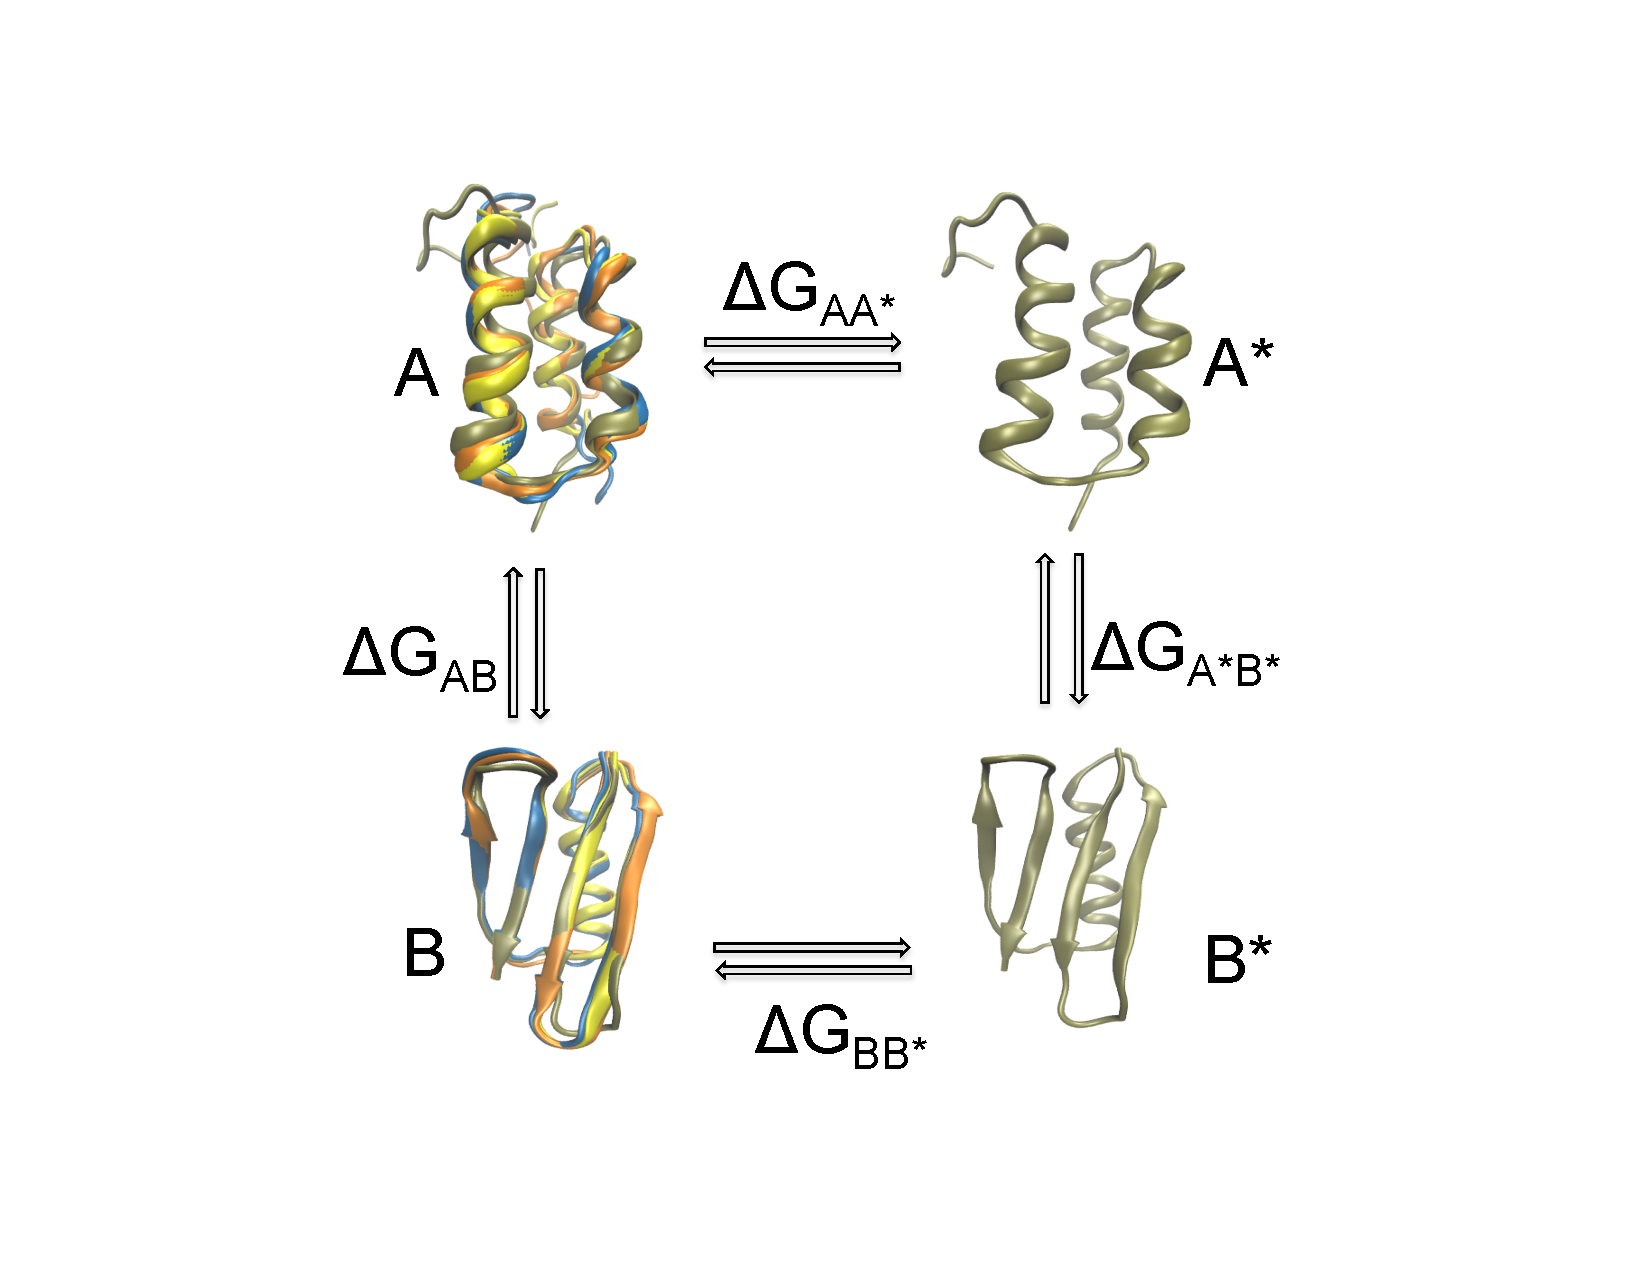
\includegraphics[width=3.5 in]{method.pdf}
    \end{center}
    \caption{Graphical representation of the thermodynamic cycle employed in the confinement method.}
\label{fig:method}
\end{figure}

Previously, the confinement method has been validated on small model peptides~\cite{Tyka2006,Cecchini2009}. Here, we
show that the confinement method can also be applied successfully to larger systems, such as the series of chameleon
proteins designed by Orban and co-workers~\cite{Alexander2007,He2008,Alexander2009,Bryan2010,He2012}, which can switch
between two completely different folds with only slight changes in sequence. We also show that our computed difference
free energies are useful in evaluating the quality of CASP target protein predictions.  This could ultimately be of significant
value for improving the energetics in protein-structure models, not just the structures. And, finally, we
show that we can approximately decompose difference free energies into individual amino acid components. This offers the
opportunity for diagnosing the structural basis for difference free energies, which may be useful for interpreting
biological mechanisms.

\section*{Results and Discussion}

\subsection*{The confinement method succeeds at some basic consistency checks}

First, we verified that our implementation of the confinement method produces results compatible with
calculations previously reported in the literature. The method has been applied to a 16 amino acid residue
$\beta$-hairpin from protein G, known as BHP~\cite{Cecchini2009}. We calculated the free energy difference between the
native conformation (called bhp1, which has a two-stranded $\beta$-sheet) and a non-native conformation (called bhp3,
which has a three-stranded $\beta$-sheet). Our confinement calculation shows that bhp1 is more stable by 1.7 kcal/mol,
which is consistent with 200 $\mu$s equilibrium simulations showing that bhp1 is favored by 1.8
kcal/mol, and also in agreement with previous calculations~\cite{Cecchini2009}.

Second, we looked at 6 target proteins from the CASP9 experiment~\cite{Moult2011}. For each target, we examined up to 5
submitted models.  We computed the difference free energy between the experimental native structure and the best model.
Figure~\ref{fig:summary_casp} and Table~\ref{table:casp_control} show that, in 5 out of 6 cases, the confinement method
assigns a lower free energy to the experimentally determined structure than to any of the decoys. Other well-known
discriminators can also successfully tell native structures from computer generated models~\cite{Sheffler2009,Zhou2002};
providing independent validation that the confinement calculations make sense.

\begin{table}
\begin{center}
\caption{The confinement method assigns a more favorable free energy to the experimentally determined structure than to
    computer-generated predictions. For each target, we examined as many as five predictions submitted by CASP
    participants. We report the free energy difference between the most favorable decoy and the experimentally
    determined structure. Positive $\Delta\Delta G (=\Delta G_{best~decoy} - \Delta G_{native})$ values indicate that
    the experimental structure is predicted to be more favorable than any of the decoys.}
\label{table:casp_control}
\begin{tabular}{l l l l}\hline
    CASP Target  & PDB Identifier & $\Delta \Delta G$ (kcal/mol) & GDT-TS \\ \hline
     T0531       &    2KJX        &          $11.15 \pm 0.70$    &  $44$ \\ \hline
     T0538       &    2L09        &          $-3.00 \pm 0.47$    &  $96$ \\ \hline
     T0540       &    3MX7        &          $16.94 \pm 0.49$    &  $70$ \\ \hline
     T0559       &    2L01        &          $2.10 \pm 0.24$     &  $94$ \\ \hline
     T0560       &    2L02        &          $18.00 \pm 0.49$    &  $94$ \\ \hline
     T0569       &    2KYW        &          $20.01 \pm 0.69$    &  $78$ \\ \hline
\end{tabular}
\end{center}
\end{table}

\subsection*{The confinement method correctly predicts the structures of chameleon sequences}

We also tested the confinement method predictions for difference free energies on the chameleon sequences of Orban et
al.\cite{Alexander2007,He2008,Alexander2009,Bryan2010,He2012}. These are instances in which two highly similar sequences
fold into remarkably different structures. Orban and co-workers have designed a protein-G-like sequence of 56-residues
that is marginally stable in one of two possible folds. By mutating key residues in this sequence, they are able to
stabilize one fold or the other (see Figure~\ref{fig:orban}). We refer to the $4\beta + \alpha$ structure as the $\beta$
conformation, and we refer to the $3\alpha$ structure as the $\alpha$ conformation. We denote sequences that prefer the
$\alpha$ fold as GA and sequences that prefer $\beta$ as GB. One pair of sequences (GA88/GB88) is 88 percent identical
in sequence, differing in seven positions. Another pair (GA95/GB95) is 95 percent identical, differing in three
positions. Accurately predicting the structural preferences of such similar sequences poses a difficult challenge for
computational methods \cite{Allison2011}.

%The phrase "protein data bank identifier" is a bit confusing. I can't tell if it means the abbreviation that identifies the structure, or if you mean the structure. If you mean the experimentally determined structure, then I suggest saying "the structure determined by nmr/x-ray crystallography." I suppose that you will want to give the resolution of the experimental structures somewhere...

\begin{figure}
    \begin{center}
    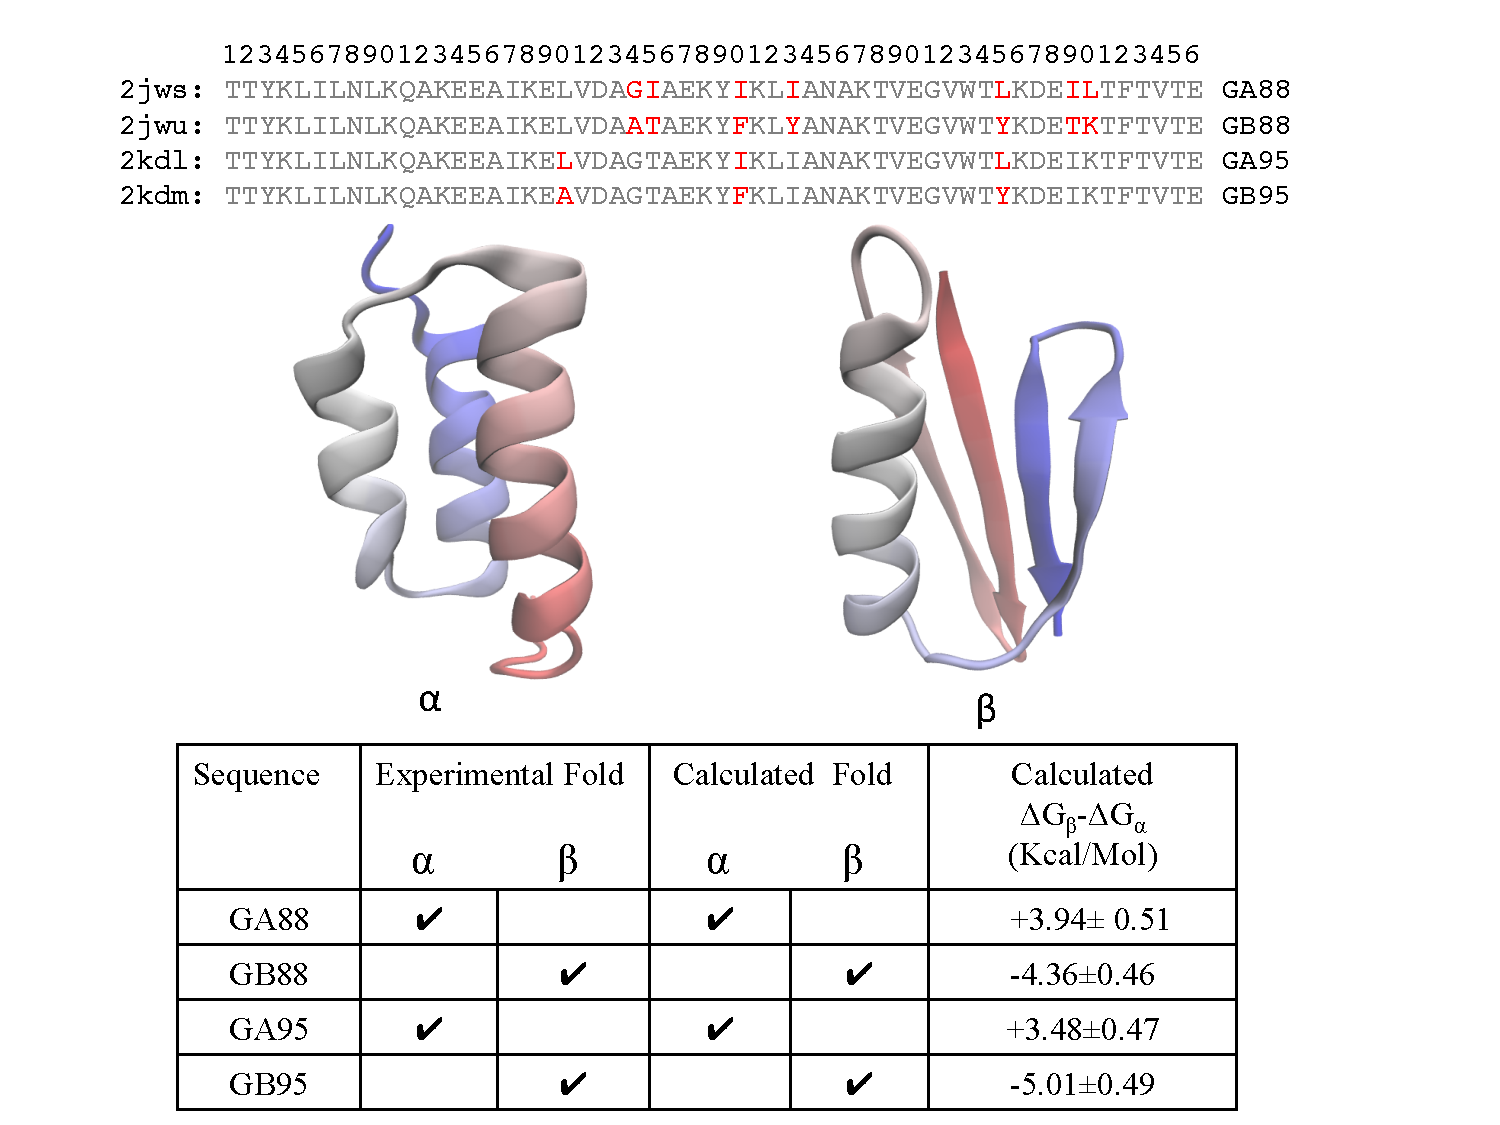
\includegraphics[width=5.0in]{orban.pdf}
    \end{center}
    \caption{The confinement method correctly predicts the structural preferences of four chameleon sequences. The top
        part of the figure represents four sequences used in this study along with the protein data bank identifier. The
        experimentally observed fold, computationally predicted fold, and difference free energy between the two folds
        is reported for each sequence.}
\label{fig:orban}
\end{figure}

We initially approached this problem by making a model of each sequence with the same backbone structure as its partner
chameleon sequence. For example, we took the sequence of GA88 and built a model with the same overall structure as GB88.
We then used the confinement method to assess the free energy difference between these two structures. In other words,
we compared the experimentally determined GA88/$\alpha$ structure with the computer-generated GA88/$\beta$
structure. The confinement method predicted the conformational preferences correctly for all four sequences
(data not shown). This is, however, not surprising as it is often easy to distinguish computational models from native
structures~\cite{Handl2009,Sheffler2009}. To better test our method, we instead computed the relative free energies of
two different computer generated models for each sequence. One model is based on the $\alpha$ structure and the other on
the $\beta$ (see Supporting Information for details on the modeling procedure). This is a more stringent
test of the confinement method's accuracy in predicting the difference free energy.

Figure~\ref{fig:orban} shows that the confinement method identified the correct structure for all four sequences. One
hypothesis is that such structural transitions require states with diminished stability~\cite{Bryan2010}. It is believed
that if the free energy of the native state and the alternative state are within a range of around 5 kcal/mol, then it
is possible for the native state to be destabilized relative to the alternative state with only small changes in
sequence~\cite{He2008,Alexander2009,Bryan2010}. The calculated free energy differences range from around 3.5 to 5.0
kcal/mol, which is consistent with this hypothesis. In a more recent study\cite{He2012}, the amino acid residue at
position 45 (Tyr for $\beta$ and Leu for $\alpha$) was found to be important for switching between $\alpha$ and $\beta$
conformations. This inspired us to introduce another mutation at this position, Y45A, which we refer to as GA98. Our
calculations predicted that this mutation shifts the equilibrium to the $\alpha$ conformation, which is now more stable
than the $\beta$ by 3.8 kcal/mol. Although this result has not yet been confirmed experimentally, it is
consistent with the previously observed effect of Y45L.

\subsection*{Per-residue free energy calculations can identify mechanistic details behind conformational preferences}

To better understand the switching mechanism of these chameleon proteins, we approximately decomposed~\cite{Tyka2006} the free
energy into per-residue contributions to each confinement step ($\Delta G_{A,A^\ast}$, $\Delta G_{B,B^\ast}$). 
We can also decompose the remaining enthalpy in the confined ensemble into per-residue
contributions. However, the method is approximate because we do not include the residual conformational entropy from the
normal mode or quasi-harmonic analysis steps. Computing per-residue contributions helps us to identify important residues
that stabilize a particular conformation. The per-residue difference free energy, $\Delta \Delta G (\beta - \alpha)$, is
shown in Figure~\ref{fig:perresidue_orban}.

\begin{figure}
    \begin{center}
        \includegraphics[width=4.5in]{delta_g.pdf}
    \end{center}
    \caption{Per-residue difference free energies for the $\alpha$ and $\beta$ conformations of the GA95 and GB95
        sequences. Residues colored in blue favor the $\alpha$ structure; residues in red favor the $\beta$ structure;
        and white residues have no preference.}
\label{fig:perresidue_orban}
\end{figure}

Although the overall free energy difference between the two structures is small (within 3--5 kcal/mol), individual
residues can show marked preferences for being in either $\alpha$ or $\beta$ conformation. Such differences can be
understood by looking at the details of the local environments for those residues. For example, the region around residue 7
forms a random coil in the $\alpha$ structure, whereas it forms a beta-sheet structure in the $\beta$ structure. These
residues strongly favor the locally well-packed and hydrogen bonded environment found in the $\beta$ sheet, but in the
alpha conformation there are no other residues to form a beta sheet with. The global conformation of the protein has
"overridden'' the local preference of these residues. Overall, favoring the $\alpha$ or $\beta$ structure is a delicate
balance, where the global free energy difference is small, and the contributions of different per-residue tendencies
largely cancel out. For these chameleon proteins, it is therefore very likely that the global
fold preferences can be changed by changing key residues.

Three residues are mutated between GA95 and GB95, at positions 20, 30, and 45. In GA95, these residues (L20, I30 and
L45) stabilize the $\alpha$ structure (Figure~\ref{fig:perresidue_orban}, upper panel). In GB95 (lower panel), two of
these residues (F30 and Y45) favor the $\beta$ structure, because they have large solvent exposed surface areas in the
$\alpha$ structure, while they are more buried in the $\beta$ structure. Additionally, Y45 forms a hydrogen bond with D47 in
the $\beta$ structure. On the other hand, residue A20 from GB95 still favors the $\alpha$ structure, although less
strongly than L20 in GA95.

The GA and GB sequences are nearly identical, so there are some common features observed for all sequences.
The experimental observations classified the protein into two parts: Amino acids 9--51 are fully structured in both
folds, whereas residues 1--8 and 52--56 are unstructured in the $\alpha$ fold, but form $\beta$-strands in the $\beta$
fold. Most of the amino acid residues in the 
%structured?
region 1--9 have negative per-residue free energies, which means that these
residues favor the $\beta$ structure. Roles of some other important residues in stabilizing either the $\alpha$ or
$\beta$ conformation are summarized in Figure S1.

In addition to the direct effects of the mutation, there are also indirect effects due to small perturbations in the
environment around the mutations. For example, the L20A mutation causes a slight repacking around residue 20. This
causes large changes in the per-residue free energies of nearby residues T25 and A26. However, the changes for these two
residues have opposite signs and nearly cancel.

These per-residue free energy decompositions provide a great deal of insight into the driving forces behind protein
folding and conformational change. We believe that such calculations may also be useful for designing proteins with
specific structures and functions.

\subsection*{The confinement method is a useful tool for structure prediction}

Having tested the ability of the confinement method to act as a "meta-predictor'' for structure prediction, the next
task was to correctly identify the most accurate models out of a set of "decoys'' generated by different methods during
the CASP experiment. CASP is a blind test in which different groups apply computational methods to predict the 3-dimensional structures
of proteins from their sequences. Each group is allowed to submit five possible structures, ranked by that group from best to worst.

We performed two experiments based on CASP. In the first experiment, we tried to rank-order predictions for
several targets. For each target, the predictions were either produced by a single group�presumably using the same
method for each prediction, or were produced by several different groups�using different methods. The goal of this
experiment was to determine if the physics-based confinement method could correctly identify more native-like structures as
having lower free energies. Our second experiment was to see if the confinement method could identify structures that are
missed by other meta-prediction servers. Most successful meta-prediction servers are based on the idea of consensus: if
many different prediction methods produce similar results, then that is probably a correct prediction
\cite{Kryshtafovych2011,Wang2011}. This is often a powerful heuristic, but it can miss cases where there is a very good
result that is only predicted by one method. We chose several cases where such structures were missed by the best
meta-predictors in CASP and assessed if the confinement method could correctly identify these accurate models. All of our
calculations were performed after the CASP experiment; they were not blind predictions.

As is common in the CASP experiment, we assess our results in terms of Global Distance Test Total Score (GDT-TS)
\cite{Zemla2003}, which is a C$\alpha$ based measure of structural accuracy. It can be understood roughly as the
percentage of residues that are correctly positioned in the model (range 0 to 100, higher is better). We did not have
enough computer power to analyze every model, so we chose a small subset of examples from a selection of different
server groups that have done well in past CASP events.

Overall, the confinement method performs well on our CASP tests. Figure~\ref{fig:summary_casp} shows that in almost
every case, the native structure has the lowest free energy and the best model has the next lowest free energy. The
confinement method appears to be a useful tool for ranking structure predictions.

\begin{figure}
\begin{center}
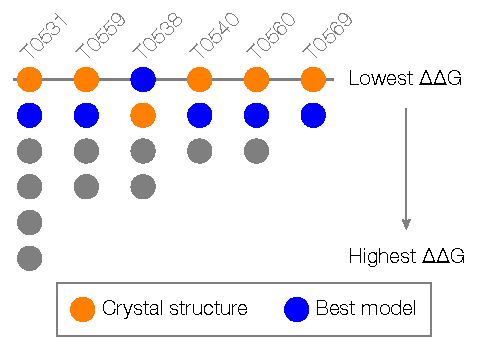
\includegraphics[width=3.5 in]{casp.pdf}
\end{center}
\caption{The confinement method is usually able to identify the native structure and the best model (the model with the
    highest GDT-TS) from a set of decoys.}
\label{fig:summary_casp}
\end{figure}

\subsection*{The confinement method can correctly rank-order structure predictions}

First, we examined the ability of the confinement method to rank different models  generated
by a single group using the same methodology for all predictions. We examined two targets: T0559 and T0560 (see
Table~\ref{table:casp_testcase}).


\begin{table}
\begin{center}
\caption{The six different CASP targets that are used in this study. The corresponding PDB Identifier and description
    are also listed.}
\label{table:casp_testcase}
\begin{tabular}{l l l}\hline
    CASP Target  & PDB Identifier &  Description \\ \hline
     T0531       &    2KJX        &  extracellular domain of the jumping  \\
                 &                &  translocation breakpoint protein  \\ \hline
     T0538       &    2L09        &  protein asr4154 from Nostoc sp. PCC7120     \\ \hline
     T0540       &    3MX7        &  human Fas apoptotic inhibitory molecule     \\ \hline
     T0559       &    2L01        &  protein BVU3908 from Bacteroides vulgatus   \\ \hline
     T0560       &    2L02        &  protein BT2368 from Bacteroides  \\
                 &                &  thetaiotaomicron         \\ \hline
     T0569       &    2KYW        &  domain of adhesion exoprotein from \\
                 &                &   Pediococcus pentosaceus \\ \hline
\end{tabular}
\end{center}
\end{table}


The first test case is target T0559. The best predictor group for this 69 amino acid target was "BAKER-ROSETTASERVER''.
To save computer time, we excluded two models that were very similar to other models that we did include. For this
target, the difference free energy computed by the confinement method could be used to accurately rank-order all of the
models and the native experimental structure (Figure~\ref{fig:T0559}).

\begin{figure}
    \begin{center}
        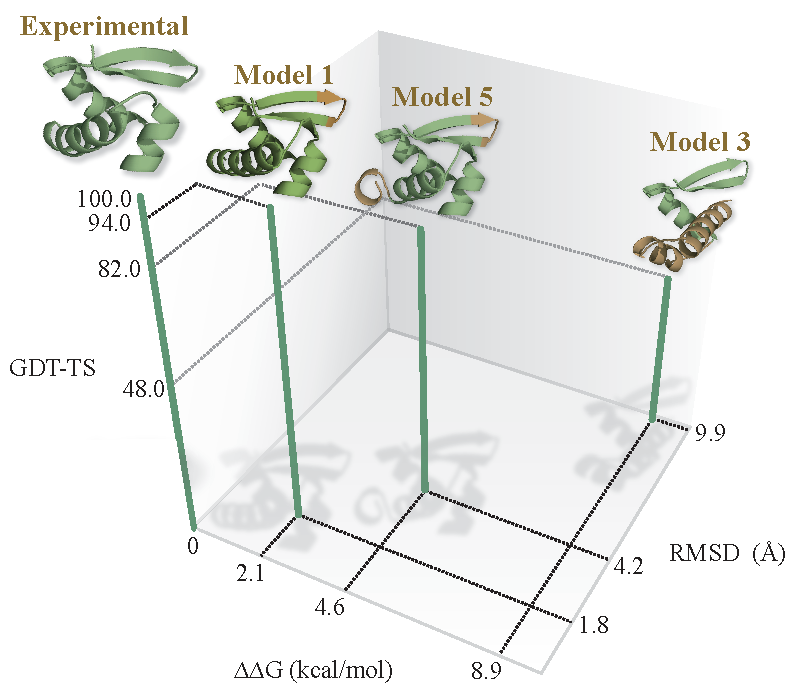
\includegraphics[width=3.8 in]{T0559.pdf}
    \end{center}
    \caption{The confinement method can correctly rank the native structure and three predictions produced by a single
        method for target T0559. The backbone regions of the predicted structures that differ substantially from the
        experimental structures upon superposition are colored brown.}
\label{fig:T0559}
\end{figure}

We performed a similar calculation for target T0560 with two models from the group "Splicer''. The remaining three
models were discarded as they were too similar to the rest of the models. Again, we can correctly identify the native
state, and our calculated free energy based ranking matches well with GDT-TS (Figure S2 in the supporting information).

Next, we tested the ability of the confinement method to rank the models for target T0540 that were produced by different
prediction groups. The top models from groups "LTB'' (Model 1) and "Mufold'' (Model 2) were chosen for analysis. Once
again, the free energy based ranking correlates well with the GDT-TS based score (Figure~\ref{fig:T0540}).

\begin{figure}
    \begin{center}
        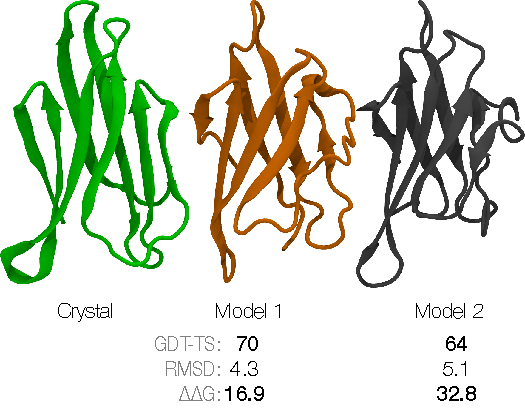
\includegraphics[width=3.5 in]{T0540.pdf}
    \end{center}
    \caption{The confinement method can correctly rank the native structure and two models submitted by different
        prediction groups.}
\label{fig:T0540}
\end{figure}

\subsection*{The per-residue free energy is sensitive to small changes in protein conformation}

We discussed how the per-residue free energy can reveal mechanistic detail behind the
conformational preference of chameleon sequences. Here, we applied the same method to
see if the per-residue free energy can help us identify problematic residues in structure predictions. We chose
CASP target T0569 and compared the experimental NMR structure with the best predicted model (GDT-TS=78; predicted by the
"Mufold'' group). The confinement method predicts that the experimental structure is more stable by 20 kcal/mol (Figure
S2).
%The annoying rule is that "side chain" is correct for the noun usage, and side-chain for the adjective.
The confinement method clearly identified the two hydrophobic residues V59 and I61as destabilizing the predicted model
relative to the experimental structure (Figure~\ref{fig:T0569_per_residue} and Figure S3). The side chains of these
hydrophobic residues are oriented towards the protein hydrophobic core in the native NMR structure but are oriented towards
the exterior of the protein, exposing them to solvent, in the model. These residues are part of a beta-sheet in the
experimental structure, but because of their side-chain orientation, the corresponding beta-sheet becomes disordered in
the predicted model (Figure~\ref{fig:T0569_per_residue} and Figure S4). There is also a large difference around K76,
which forms a salt-bridge with D11 in the predicted model, but not in the experimental structure. This suggests that
salt-bridge interactions are too favorable for the combination of forcefield and implicit solvent model we use, which
has been a problem noted in the past \cite{Roe2007}.

\begin{figure}
    \begin{center}
        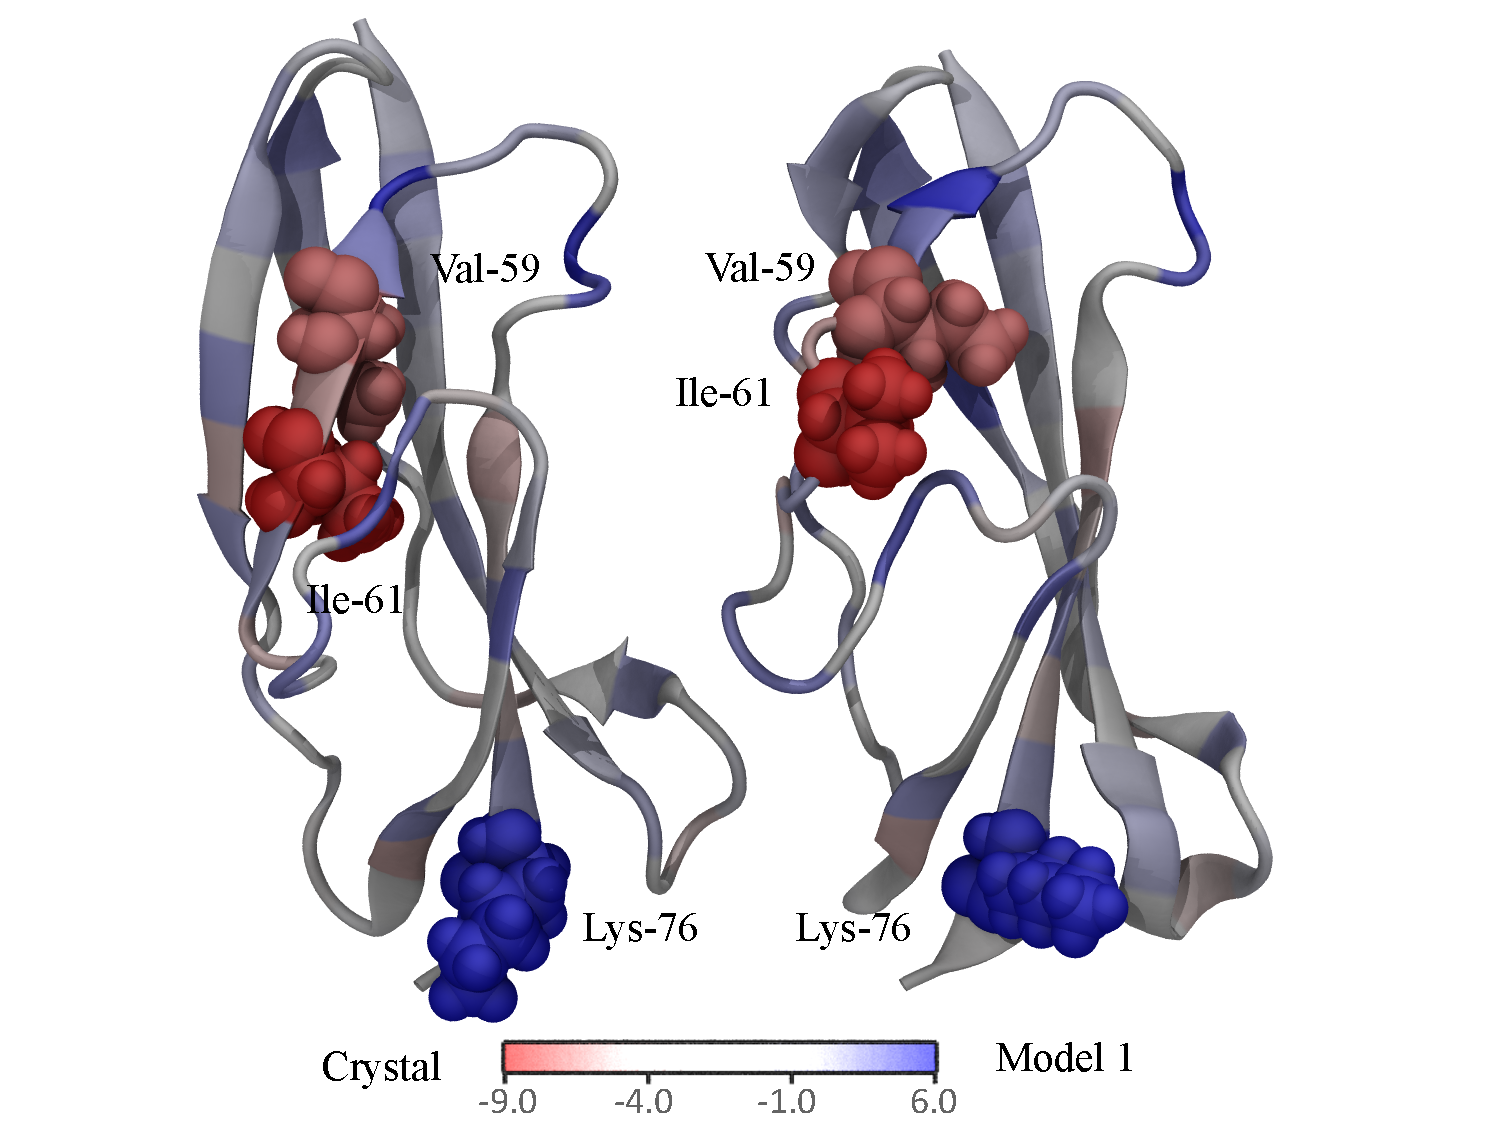
\includegraphics[width=3.5in]{T0569_perres1.pdf}
    \end{center}
    \caption{Per-residue difference free energy between the experimental NMR structure and the best prediction for CASP
        target T0569. The amino acid residues that are colored in deep red and deep blue stabilizes the NMR structure
        and the prediction, respectively; the residues with light blue color do not have a strong preference.}
\label{fig:T0569_per_residue}
\end{figure}

\subsection*{The confinement method occasionally produces incorrect results}

Despite success for most of the systems we studied, there were few failures, especially when the GDT-TS scores of the
compared structures were very close. One example is Target T0538, where we compared the experimental structure with three
models (Model 1: "PconsR''---GDT-TS=96; Model 2: "Shell''---GDT-TS=90; Model 3: "FOLDIT''---GDT-TS=86). Contrary to
our expectation, the confinement method predicts that computer generated Model 1 is more stable than the crystal
structure (Figure S5). Per-residue free energy calculations (not shown) show that despite only small variations at the
backbone level, the side chains are oriented in very different ways (Figure~\ref{fig:T0538compare}), giving rise to
large differences in the stabilization of certain residues. In particular, some of the differences arise from different
salt bridge patterns and certain flexible polar residues exposed to the surface. This unexpected result shows that the
confinement method is very sensitive to local interactions (including side chain reorientation) and may indicate issues
with the forcefield and implicit solvent models used in the calculation.


\begin{figure}
\begin{center}
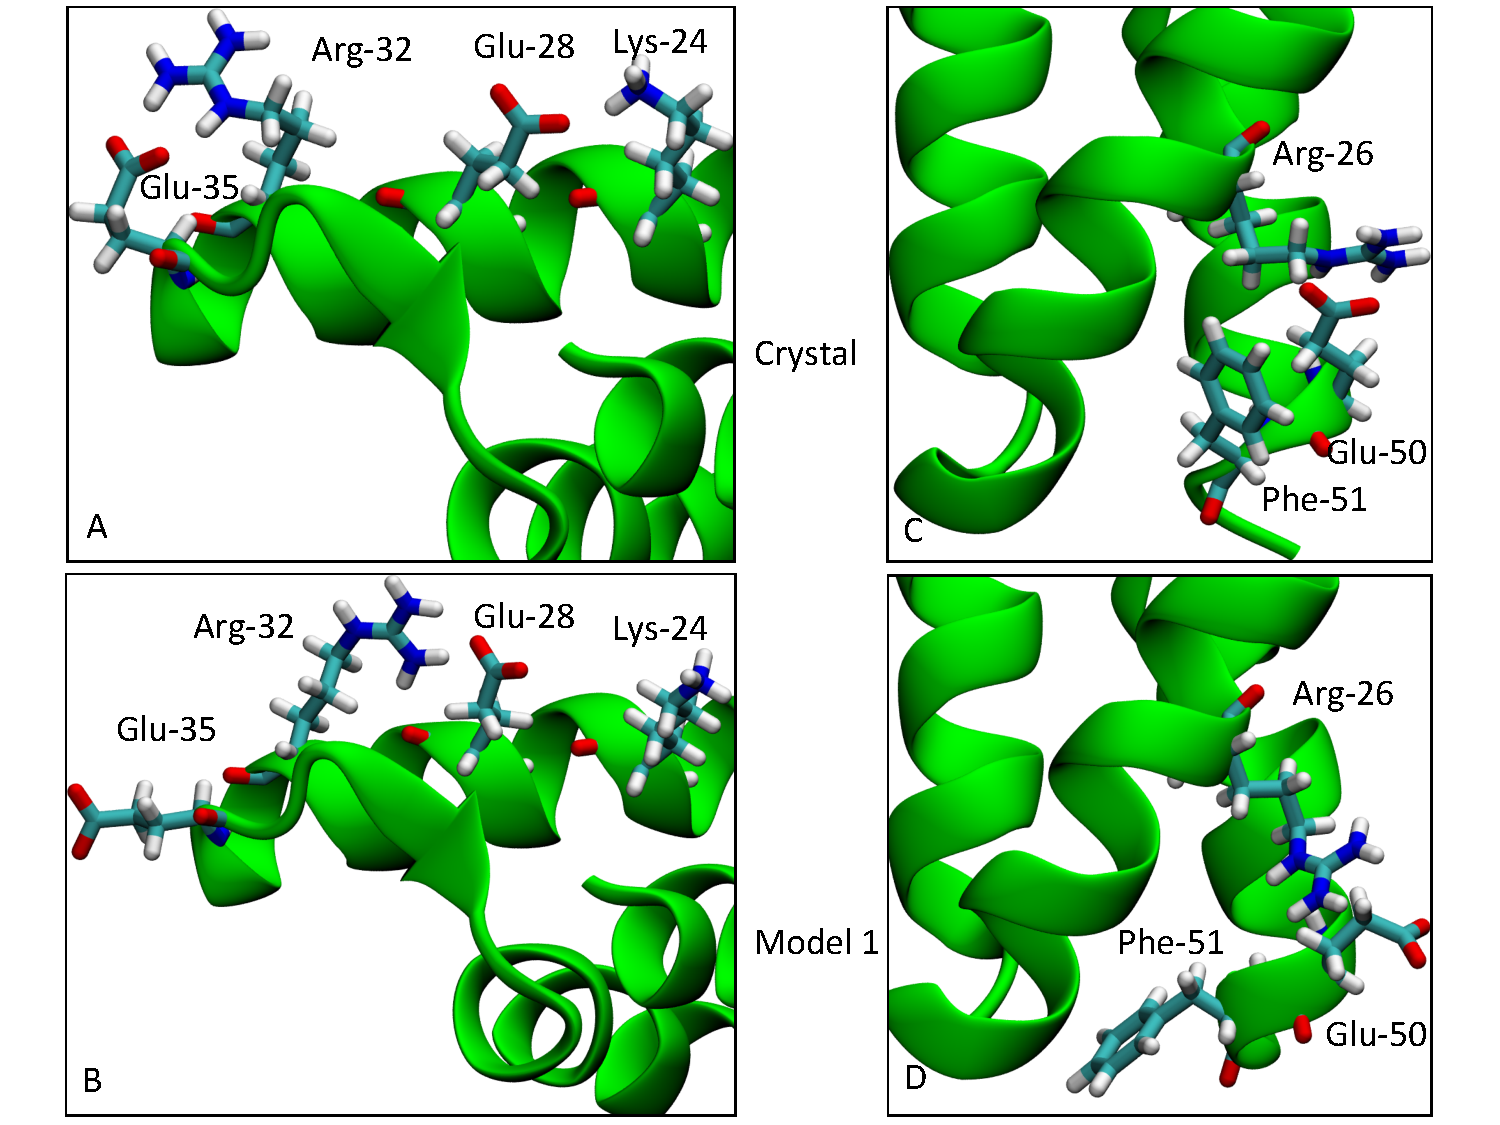
\includegraphics[width=4.9 in,height=4.0 in]{Target_538_compare.pdf}
\end{center}
\caption{Small differences in side-chain orientation can cause large differences in free energy. We compare the
    experimental structure and a computer generated model for CASP target T0538. (A) Two salt bridges between residues
    E35-R32 and E28-K24 exist in the native structure. These are absent in the computer generated model structure.
    Instead, (B) a new salt bridge is formed between residues R32-E28 in model. (C) Another salt bridge between residues
    R26-E50 in the experimental structure. (D) In comparison to the native structure, orientation of F51 differs in the
    model.}
\label{fig:T0538compare}
\end{figure}


\subsection*{Can the confinement method improve the assessment of quality in protein structure prediction?}

A part of the CASP experiment is dedicated to the quality assessment (QA) of predicted models \cite{Kryshtafovych2011}.
Predictors are asked to produce an overall score (called QMODE1) for each model on a scale from 0 to 1, with
higher values corresponding to better models \cite{Kryshtafovych2011}. Many of the groups use consensus strategies in
such experiments. Here, we chose two computer generated models from CASP target T0538, where the top performing group
"MUFOLD-WQA'' \cite{Wang2011} failed to identify the best model. We examined two models, one from "PconsR'' (GDT-TS =
96), which MUFOLD-WQA gave a QMODE1 = 0.54. The second model was from "MULTICOM-NOVEL'' (GDT-TS=83), which is a poorer
model, but MUFOLD-WQA assigned a higher QMODE1 = 0.59. The confinement method gave a difference free energy that favored
the PconsR model by 3.9 kcal/mol, which correctly identified the more accurate model. Although consensus prediction
strategies are very effective, they can miss a good prediction if it is predicted by only a few methods. At least in this
case, the confinement method was able to capture a structure that was otherwise missed.

\section*{Conclusion}

We have described a computational method called the confinement method for computing the difference free energy between
two conformational ensembles. We showed that the difference free energy can be calculated on proteins of ~100 residues,
even for large conformational changes; that it can discriminate the folding preferences of a series
of chameleon proteins; it can discriminate between the native structure and structure
predictions, and can identify the best prediction reliably. Perhaps most importantly, we have shown that it can be used
to give residue-level insights into the dominant structural factors that are responsible for the
difference free energies in conformations of a protein. The confinement method should be useful for protein design, structure prediction, and understanding
the mechanism of conformational change.


\section{Method}

The confinement method has been described in detail by Tyka et al. in reference \cite{Tyka2006} and Cecchini et al.
\cite{Cecchini2009}. The basic approach of the confinement approach is the same in both these papers. A thermodynamic
cycle is used to compute the free energy between conformations A and B. However, there are some small technical
differences between the two approaches. Here, we briefly describe the procedure that we used.

\begin{enumerate}

\item  In the first step, minimizations of A and B conformations are performed. These minimized conformations
    ($A^{\ast}$ and $B^{\ast}$) are the reference conformations.
% I changed et. al. to et al for consistency.
\item The free energy of confining the ensemble (A or B) to a tighter ensemble ($A^\ast$ or $B^\ast$) is calculated.
    This is done by gradually confining each atom to its position in the reference conformation ($A^{\ast}$ or
    $B^{\ast}$) using a series of progressively stronger position restraints. This is done by running 21 molecular
    dynamics simulation (each 20 ns long) for each leg of the thermodynamic cycle, where the harmonic restraint force
    constant is scaled from 0.00005 kcal/mol (mostly free) to 81.92 kcal/mol (tightly restrained). The free energy for
    this step is estimated using a thermodynamic integration approach developed by Tyka et al \cite{Tyka2006}. The
    confinement free energies calculated in this step are denoted as $\Delta G_{A,A^\ast}$ and $\Delta G_{B,B^\ast}$ in
    Figure~\ref{fig:method}.

\item The thermodynamic cycle is closed by calculating the free energy between the final restrained states $A^\ast$ and
    $B^\ast$ using normal mode analysis \cite{Brooks1983,Case1994} or quasi-harmonic analysis
    \cite{Karplus1981,Levy1984}. The free energy calculated in this way is shown as $\Delta G_{A^\ast,B^\ast}$ in
    Figure~\ref{fig:method}.

\item  The full free energy, $\Delta G_{A,B}$ between the two state A and B is calculated as
    $\Delta G_{A,B} = \Delta G_{A,A^\ast} - \Delta G_{B,B^\ast} + \Delta G_{A^\ast,B^\ast}$.

\end{enumerate}

One advantage of the confinement method is that none of the simulations during the restraining step depends on any other.
Therefore, it can be fast to compute with available computer resources. We ran each confinement calculation on a single
graphics processing unit (GPU). For a 56-residue protein, this leads to a calculation time of only 4 hours on 40 GPUs (1
GPU per confinement calculation x 20 calculations per structure x 2 structures). All calculations were performed with
the Amber 11 suite of programs~\cite{Case2012,Goetz2012} in combination with the ff99SB forcefield~\cite{Hornak2006} and
the GBneck generalized born implicit solvent model \cite{Mongan2006}.

We calculated the approximate per-residue free energy as follows. The confinement energy, $\Delta G_{A,A*}$ and $\Delta
G_{B,B*}$ of each residue was calculated numerically as described by Tyka et al. \cite{Tyka2006}. The
internal energy of each residue was calculated with Amber's "decomp" module using the final restrained trajectory. We
call this method approximate as we ignore the entropic contribution from the normal mode or quasi-harmonic analysis.
However,
% the entropic
contribution to the total free energy is much smaller, which allow us to study the details of
the conformational preferences of each residue.

\begin{thebibliography}{99}
%You may want to check your styles for creating the references against the style of the Journal to which you are submitting the paper. Also, you may want to check your abbreviations for some of the journal titles against a list such as the one at: http://library.caltech.edu/reference/abbreviations/.  E.g. J. Chem. Phys. or J Chem Phys...Proc. Natl. Acad. Sci. U.S.A. or Proc. Natl. Acad. Sci. 
\bibitem{Elber2007}
Elber, R. A. Milestoning Study of the Kinetics of an Allosteric Transition: Atomically Detailed Simulations of Deoxy Scapharca
Hemoglobin. Biophysical J., 2007, 92, 85-87.

\bibitem{Moult2011}
Moult, J.; Fidelis, K.; Kryshtafovych, A.; Tramontano, A. Critical assessment of methods of protein structure prediction (CASP)-round IX.
Proteins, 2011, 79, 1-5.

\bibitem{West2007}
West, A.M.; Elber, R.; Shalloway, D. Extending molecular dynamics time scales with milestoning: example of complex kinetics
in a solvated peptide. J Chem Phys. 2007, 126, 145104-1451014.

\bibitem{Haas2007}
Haas, K.; Chu, J.W. Decomposition of energy and free energy changes by following the flow of work along reaction path.
J. Chem. Phys. 2009, 131, 144105-144111.

\bibitem{Jonsson1998}
J\'{on}sson, H.; Mills, G.; Jacobsen, K.W. Nudged Elastic Band Method for Finding Minimum Energy Paths of Transitions
in Classical and Quantum Dynamics in Condensed Phase Simulations, Ed. B. J. Berne, G. Ciccotti and D. F.
Coker, 385 (World Scientific, 1998).

\bibitem{E2007}
%Is E, W.; an error?
E, W.; Ren, W.; Vanden-Eijnden, E. Simplified and improved string method for computing the minimum energy paths in
barrier-crossing events. J. Chem. Phys. 2007, 126, 164103.

\bibitem{Dellago2002}
Dellago, C.; Bolhuis, P.G.; Geissler, P.L. Transition Path Sampling, Adv. Chem. Phys. 2002, 123, 1-84.

\bibitem{Cheng2006}
Cheng, X.; Wang, H.; Grant, B.; Sine, S.M.; McCammon, J.A. Targeted Molecular Dynamics Study of C-Loop Closure
and Channel Gating in Nicotinic Receptors. 2006, 9, 134.

\bibitem{Elber2005}
Elber, R. Long-timescale simulation methods. Cur. Opin. in Str. Biol. 2005, 15, 151-156.

\bibitem{Chipot2007}
Chipot, C.; Shell, M.S.; Pohorille, A. Introduction, in Chipot, C., Pohorille, A., editors. Free Energy
Calculations: Theory and Applications in Chemistry and Biology. Springer Series in Chemical
Physics, vol. 86. Berlin and Heidelberg: Springer; 2007, p. 1–32.

\bibitem{Torrie1977}
Torrie, G. M.; Valleau, J. P. Nonphysical sampling distributions in Monte Carlo free-energy estimation: Umbrella sampling
(1977) J. Comput. Phys. 23, 187

\bibitem{Mascarenhas2013}
Mascarenhas, N. M.; Kastner, J. How maltose influences structural changes to bind to maltose-binding protein: Results from umbrella sampling simulation. Proteins. 2013, 81, 185-198.

\bibitem{Kumar1992}
Kumar, S.; Rosenberg, J.M.; Bouzida, D.; Swendsen, R.H.; Kollman, P.A. The weighted histogram analysis method for free-energy calculations on biomolecules. I. The 
method. J Comput Chem. 1992, 13, 1011-1021.

\bibitem{Ytreber2006a}
Ytreberg, F.M.; Swendsen, R.H.; Zuckerman, D.M. Comparison of free energy methods for molecular systems. J Chem Phys. 2006, 125, 184114.

\bibitem{Ytreberg2006}
Ytreberg, F.; Zuckerman, D. Simple estimation of absolute free energies for biomolecules. J. Chem. Phys. 2006, 124, 104105.

\bibitem{Park2008}
Park, S.; Lau, A.; Roux, B. Computing conformational free energy by deactivated morphing. J. Chem. Phys. 2008, 129, 134102

\bibitem{Zheng2008}
Zheng, L.; Chen, M.; Yang, W. Random walk in orthogonal space to achieve efficient free-energy simulation of complex systems, Proc. Natl. Acad. Sci. 2008, 105 (51), 20227.

\bibitem{Shell2010}
Shell, S.M. A replica-exchange approach to computing peptide conformational free energies. Mol. Sim. 2010, 7, 505-515.

\bibitem{Tyka2006}
Tyka, M.; Clarke, A.; Sessions, R. An Efficient, Path-Independent Method for Free-Energy Calculations. J.Phys.Chem. B 2006, 110, 17212-17220.

\bibitem{Cecchini2009}
Cecchini, M., Krivov, S.V., Spichty, M., Karplus, M. Calculation of free-energy differences by confinement simulations. Application to peptide conformers. J. Phys. Chem. B. 2009, 113, 9728-9740.

\bibitem{Ovchinnikov2013}
Ovchinnikov, V.; Cecchini, M.; Karplus, M. A Simplified Confinement Method for Calculating Absolute Free Energies
and Free Energy and Entropy Differences. J. Phys. Chem. B. 2013, 117, 750-762.

\bibitem{Spichty2010}
Spichty, M.; Cecchini, M.; Karplus, M. Conformational Free-Energy Difference of a Miniprotein from Nonequilibrium
Simulations. J. Phys. Chem. Lett., 2010, 1, 1922-1926.

\bibitem{Strajbl2000}
Strajbl, M.; Sham, Y.Y.; Villà, J.; Chu, Z.-T.; Warshel, A. Calculations of Activation Entropies of Chemical Reactions
in Solution. (2000) 104, 4578-4584.

\bibitem{Brooks1983}
Brooks, B. R.; Karplus, M. Harmonic dynamics of proteins: Normal modes and fluctuations in bovine pancreatic trypsin inhibitor. Proc. Natl. Acad. Sci. U.S.A. 1983, 80, 6571-6575. 

\bibitem{Case1994}
Case, D. Normal-mode analysis of protein dynamics. Curr. Opin. Struct. Biol. 1994, 4, 285-290.

\bibitem{Karplus1981}
Karplus, M.; Kushick, J. Method for estimating the configurational entropy of macromolecules. Macromolecules. 1981, 14, 325-332.

\bibitem{Levy1984}
Levy, R.; Karplus, M.; Kushick, J.; Perahia, D. Evaluation of the configurational entropy for proteins: application to molecular dynamics simulations of 
an $\alpha$-helix Macromolecules. 1984, 17, 1370-1374.

\bibitem{Mobley2007}
Mobley, D.L.; Chodera, J.D.; Dill, K.A. The combining and release method: obtaining correct binding free energies in
the presence of protein conformational change. Journal of Chemical Theory and Computation. 2007, 3, 1231-1235.

\bibitem{Mobley2012}
Mobley, D.L.; Klimovich, P.V. Perspective: Alchemical free energy calculations for drug discovery.
J. Chem. Phys. 2012, 137, 230901-12.

\bibitem{Mobley2006}
Mobley, D.L.; Chodera, J.D.; Dill, K.A. On the use of orientational restraints and symmetry corrections in alchemical
free energy calculations. J. Chem. Phys. 2006, 125, 084902.

\bibitem{Alexander2007}
Alexander, P.A.; He, Y.; Chen, Y.; Orban, J. Bryan, P. The design and characterization of two proteins with $88 \%$ sequence identity but different structure and 
function. Proc. Natl. Acad. Sci. 2007, 104, 11963-11968.

\bibitem{He2008}
He, Y.; Chen, Y.; Alexander, P.A.; Orban, J. NMR structures of two designed proteins with high sequence identity but different fold and function. Proc. Natl. Acad. Sci. 2008, 105, 14412-14417.

\bibitem{Alexander2009}
Alexander, P.A.; He, Y.; Chen, Y.; Orban, J. Bryan, P. A minimal sequence code for switching protein structure and function. Proc. Natl. Acad. Sci. 2009
, 106, 21149-21154.

\bibitem{Bryan2010}
Bryan, P.N.; Orban, J. Proteins that switch folds. Curr Opin Struct Biol. 2010, 20, 482-488.

\bibitem{He2012}
He, Y.; Chen, Y.; Alexander, P.A.; Bryan, P.N.; Orban, J. Mutational tipping points for switching protein folds and functions. Structure. 2012, 20,
83-91.

\bibitem{Sheffler2009}
Sheffler, W.; Baker, D. RosettaHoles: Rapid assessment of protein core packing for structure prediction, refinement, design, and validation. Protein Science. 2009, 18(1), 229-239.

\bibitem{Zhou2002}
Zhou H, Zhou Y. Distance-scaled, finite ideal-gas reference state improves structure-derived potentials of mean force for structure selection and
stability prediction. Protein Sci. 2002, 11, 2714-2726.

\bibitem{Allison2011}
Allison, J.R.; Bergeler, M.; van Gunsteren, W.F. Can computer modeling explain why two highly similar sequences fold into different structures ?
Biochemistry. 2011, 50, 10965-10973. 

\bibitem{Handl2009}
Handl, J.; Knowles, J.; Lovel, S.C. Artefacts and biases affecting the evaluation of scoring
functions on decoy sets for protein structure prediction. Bioinformatics, 2009, 25, 1271-1279.

\bibitem{Kryshtafovych2011}
Kryshtafovych, A.; Fidelis, K; and Tramontano, A. Evaluation of model quality predictions in CASP9. Proteins, 2011, 79, 91–106

\bibitem{Wang2011}
Wang, Q.; Vantasin, K.; Xu, D.; Shang, Y. MUFOLD-WQA: A new selective consensus method for quality assessment in protein structure prediction.
Proteins, 2011, 79: 185-195.

\bibitem{Zemla2003}
Zemla, A. LGA: a method for finding 3D similarities in protein structures. Nucleic Acids Res 2003, 31, 3370–3374.

%I think that Case2012 is the only bibitem where you have the initials before the last name; and the date in parentheses.
\bibitem{Case2012}
D.A. Case, T.A. Darden, T.E. Cheatham, III, C.L. Simmerling, J. Wang, R.E. Duke, R. Luo, R.C. Walker, W. Zhang, K.M. Merz, B. Roberts, S. Hayik, A. Roitberg, G. Seabra, J. Swails, A.W. Goetz, I. Kolossváry, K.F. Wong, F. Paesani, J. Vanicek, R.M. Wolf, J. Liu, X. Wu, S.R. Brozell, T. Steinbrecher, H. Gohlke, Q. Cai, X. Ye, J. Wang, M.-J. Hsieh, G. Cui, D.R. Roe, D.H. Mathews, M.G. Seetin, R. Salomon-Ferrer, C. Sagui, V. Babin, T. Luchko, S. Gusarov, A. Kovalenko, and P.A. Kollman (2012), Amber12, University of California, San Francisco.

\bibitem{Goetz2012}
Goetz, A.W.; Williamson, M.J.; Xu, D.; Poole, D.; Le Grand, S.; Walker, R.C. Routine microsecond molecular dynamics simulations with AMBER - Part I: Generalized
Born. J. Chem. Theory Comput. 2012, 8(5) 1542.

\bibitem{Roe2007}
Roe, D.R.; Okur, A.; Wickstrom, L.; Hornak, V.; Simmerling, C. Secondary structure bias in generalized Born solvent models: comparison of conformational ensembles 
and free energy of solvent polarization from explicit and implicit solvation. J Phys Chem B. 2007, 111, 1846-1857.

\bibitem{Case2005}
Case, D.A.; Cheatham, III, T.E.; Darden, T.; Gohlke, Luo, H.R.; Merz, Jr., K.M.;  Onufriev, A; Simmerling, C.;
Wang, B.; R. Woods, R. The Amber biomolecular simulation programs. J. Computat. Chem. (20005) 26, 1668-1688.

\bibitem{Hornak2006}
Hornak, V.; Abel, R.; Okur, A.; Strockbine, B.; Roitberg, A.; Simmerling, C. Comparison of multiple Amber force fields
and development of improved protein backbone parameters. Proteins. 2006, 65, 712-725.

\bibitem{Mongan2006}
Mongan, J.; Simmerling, C.; A. McCammon, J.; A. Case, D.; Onufriev, A. Generalized
Born with a simple, robust molecular volume correction. J. Chem. Theory Comput.
2006, 3, 156-169.


\end{thebibliography}

\end{document}

